%%%%%%%%%%%%%%%%%%%%%%%%%%%%%%%%%%%%%%%%%%%%%%%%%%%%%%%%%%%%%%%%%%%%%%
% How to use writeLaTeX: 
%
% You edit the source code here on the left, and the preview on the
% right shows you the result within a few seconds.
%
% Bookmark this page and share the URL with your co-authors. They can
% edit at the same time!
%
% You can upload figures, bibliographies, custom classes and
% styles using the files menu.
%
%%%%%%%%%%%%%%%%%%%%%%%%%%%%%%%%%%%%%%%%%%%%%%%%%%%%%%%%%%%%%%%%%%%%%%

\documentclass[12pt]{article}

\usepackage{sbc-template}

\usepackage{graphicx,url}

\usepackage[brazil]{babel}   
\usepackage[utf8]{inputenc}  

\usepackage{fancyhdr}
\pagestyle{fancy}

\fancyhead[L]{ }
\fancyhead[R]{ }


\renewcommand{\headrulewidth}{0pt}
\sloppy
\begin{document} 



\title{IOT do Coração\\ MI - Concorrência e Conectividade}

\author{Gustavo Henrique B. de Oliveira\inst{1}}
  


\address{Departamento de Tecnologia -- Universidade Estadual de Feira de Santana
  (UEFS)\\
  Caixa Postal 252 e 294 -- 44.036-900 -- Feira de Santana -- BA -- Brasil}


\maketitle


\section{Introdução}

Segundo dados da OMS(Organização Mundial da Saúde) cerca de 17,5 milhões\cite{OMS} de pessoas morrem todos os anos de doenças cardiovasculares. Isso corresponde, segundo a ONU(Organização das Nações Unidas), a aproximadamente 22\% das pessoas nascidas por ano. É uma das doenças que mais mata no mundo, apesar do grande investimento no tratamento, a melhor forma de cuidar da saúde é prevenindo. Porém no diagnostico, as pessoas não demostram visivelmente que são possíveis padecentes, isso complica o quadro, pois o acompanhamento de imediato por um profissional de saúde é muito importante. Na primeira hora esse acompanhamento é muito importante, caso passe desse tempo, as sequelas podem ser permanentes e até piorar o quadro do paciente.

Contudo, o acompanhamento do profissional de saúde se torna restrito, pois, é desconhecido o momento no qual o paciente pode sofrer um ataque e os equipamentos necessários para o acompanhamento tornam-o mais difícil. Porém, com o surgimento das tecnologias vestíveis esse acompanhamento tornou-se mais confortável. Dependendo do equipamento o paciente nem percebe que está sendo feito esse acompanhamento.

Essas tecnologias vestíveis se encontram em uma categoria muito recente, porém abrangente, de equipamentos eletrônicos chamados \textit{IOT} (Internet of Things ou Internet das coisas, em português). Tomando isso, foi desenvolvido um sistema de monitoramento de pacientes que correm risco de sofrer problemas cardiovasculares. Esse sistema basicamente obtém dados sobre o paciente monitorado através de uma pulseira inteligente, envia-os para um servidor de borda(server fog), no qual os dados são analisados e, daí, enviados para um servidor de nuvem(server cloud) que armazena estes dados para que o médico possa analisar essas informações.


\section{Fundamentação Teórica}

\subsection{Threads}

Como os servidores em funcionamento devem atender a diversos dispositivos conectados enviando, recebendo e processando informações, cada servidor deve ser capaz de fazer tais atividades sem impedir que novos usuários se conectem. Então, cada uma dessas atividades devem ser executadas paralelamente(pseudoparalelamente), ou seja, no mesmo instante no qual um cliente se conecta o servidor deve processar essa conexão enquanto recebe dados dos outros.

Um conceito muito utilizado em processamento paralelo em computação são as threads, onde cada processo pode executar no seu espaço de memória, diversas operações paralelamente. Então, neste cenário haverá diversas threads, cada uma executando sua instrução.

\subsection{Portas}

Ao conectar em uma rede, seu computador recebe um endereço ip, que funciona basicamente como um identificador. Apesar disso, mantemos diversos serviços abertos, como os que o navegador de internet utiliza. Em um computador é comum ter vários serviços como esses funcionando, porém, se temos apenas um endereço ip, como todos esses serviços funcionam ao mesmo tempo sem entrar em conflito?\cite{portas}.Para resolver tal problema, foram criadas as portas, onde cada serviço é executado em uma porta diferente.

\subsection{Sockets}

Sockets são pontos finais de um fluxo de comunicação entre processos através de uma rede de computadores. Oferece uma abstração para o desenvolvedor, pois ao receber uma conexão, o socket se encarrega de transferir essa comunicação para outra porta do servidor, permitindo que vários clientes se conectem.

\begin{figure}[!htb]
\centering
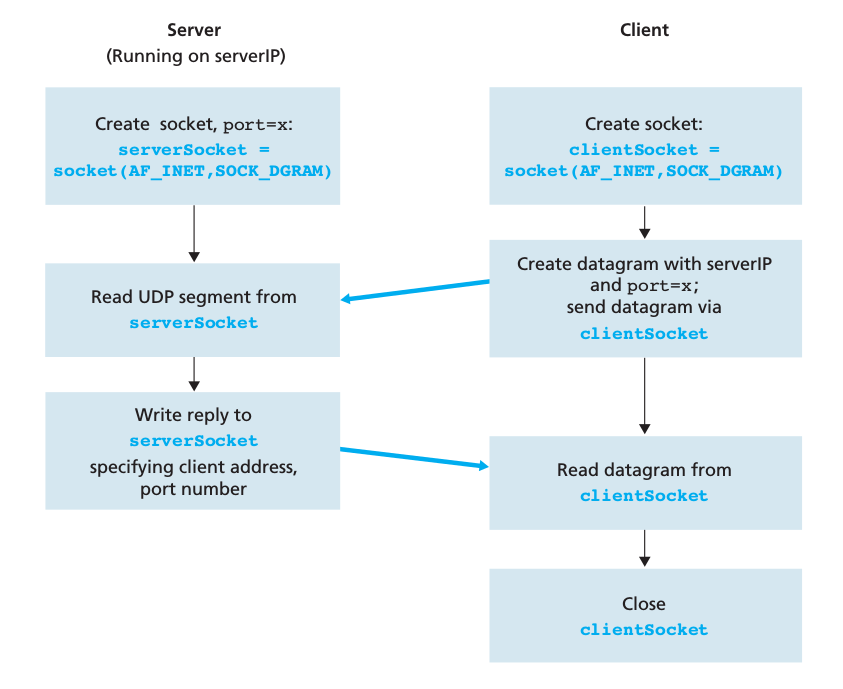
\includegraphics[scale=0.3]{pictures/udpSocket.png}
\caption{Aplicações básica cliente-servidor utilizando socket UDP.}
\label{exUdpSocket}
\end{figure}

\subsection{Protocolo de Aplicação}

Protocolo de aplicação é um padrão adotado no desenvolvimento da aplicação para o controle da conexão desses aplicativos. Permitindo que os dados enviados nessa conexão possam ser utilizados, processados e armazenados. Portanto os sensores devem enviar os dados para o servidor obedecendo esse protocolo. O servidor da mesma forma deve obedecer esse protocolo.

\subsection{Protocolo de Transporte}

O protocolo de transporte é o responsável por encapsular e transferir os dados que vão ser enviados na rede, ele independe do protocolo determinado na aplicação ou da configuração dos elementos físicos da rede. A camada de transporte reúne protocolos de transporte fim-a-fim entre as máquinas, isso significa que um sistema que implemente protocolos da camada de transporte só se comunica com o seu destinatário\cite{kurose2005computer}. Nessa camada temos diversos protocolos de transporte como o UDP e o TCP.

\subsubsection{Protocolo UDP}

O protocolo UDP é um protocolo que não é ligado a conexão\cite{kurose2005computer}, ou seja, não é necessário que haja uma conexão entre as bordas, como no TCP. Porém não é um protocolo confiável para transmissão de dados, diferente do TCP. Mas o UDP foi escolhido por conta de suas particularidades:

\begin{itemize}
\item Controle fino dos dados da camada de aplicação. O UDP vai empacotar em um segmento UDP(DatagramPacket, em Java) e passar imediatamente para a camada de rede, isso torna a troca de dados muito rápida, porém não pode-se garantir nada do recebimento. Já o TCP mantém um controle nos pacotes enviados, pois continuará enviando até que o pacote tenha chegado no seu destino, isso pode acabar congestionando a rede e o tempo no qual o pacote vai demorar para chegar ao destino é desconhecido. Além que no sistema desenvolvido os dados obtidos pelos dispositivos precisam chegar rapidamente e no caso dos dados perdidos eles não precisam ser reenviados, pois o estado atual do paciente é o que vai ser acompanhado.

\item Nenhum estabelecimento de conexão. O UDP apenas monta o pacote e passa para a camada de rede. Assim o UDP não atribui nenhum delay para estabelecer uma conexão. Diferente do TCP que utiliza handshake de três vias antes de iniciar o envio de dados.

\item Nenhum estado de conexão. O TCP mantém estado de conexões que inclui buffers de recepção e envio, parâmetros de controle de congestionamento e parâmetros de número de sequência e reconhecimento\cite{kurose2005computer}. O UDP não mantém o estado da conexão e nem rastreia nenhum desses parâmetros. Por conta disso, servidores de aplicações UDP suportam mais clientes ativos que o do TCP.

\item Sobrecarga do pacote de cabeçalho pequeno. O TCP tem 20 bytes de sobrecarga nos cabeçalhos, já o UDP possui apenas 8 bytes.
\end{itemize}

\section{Metodologia}

Para o inicio do desenvolvimento da aplicação, foi definido a arquitetura do sistema. Seguindo os comodos modos nos quais quase todas as aplicações atualmente utilizam, foi definido uma arquitetura muito simples, a cliente-servidor, figura \ref{archClientServer}. Funciona basicamente da seguinte forma.

\begin{figure}[!htb]
\centering
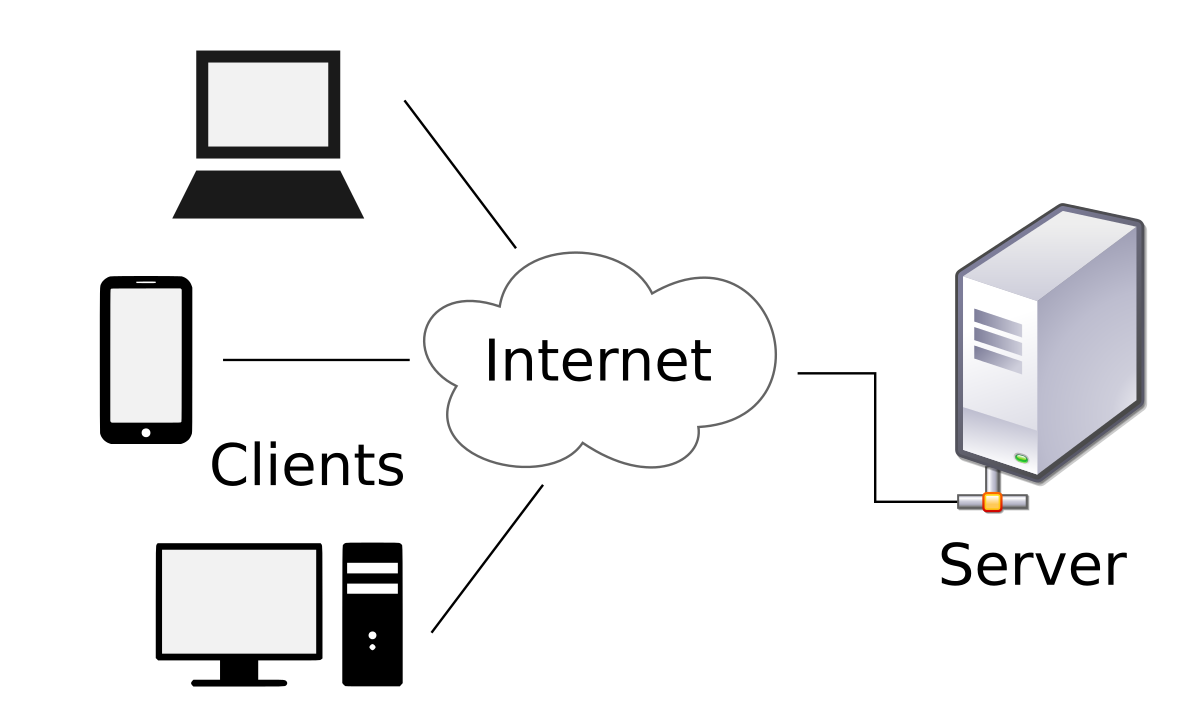
\includegraphics[scale=0.2]{pictures/architectureClientServer.png}
\caption{Arquitetura básica de aplicações cliente-servidor.}
\label{archClientServer}
\end{figure}

Basicamente o dispositivo se conecta ao servidor, a partir daí, o dispositivo passa a enviar os dados. Caso o médico queira monitorar algum paciente ele simplesmente deve se conectar ao servidor e selecionar o paciente ao qual quer obter tais dados. Porém essa arquitetura se mostrou pouco eficiente em contraste ao grande volume de dados enviados ao servidor. Por isso uma nova arquitetura precisou ser montada, com objetivo de diminuir esse grande fluxo de dados ao servidor, reduzir problemas de atrasos e excessos de dados na nuvem.

E uma arquitetura de aplicação bastante recente ajuda nisso, que é a arquitetura \textit{fog computing}, ela estende a capacidade computacional e o armazenamento da nuvem para as camadas de acesso da rede, permitindo que os dados sejam analisados e transformados em informações ou em ações antes de serem simplesmente transmitidos. É daí que vem o nome, computação em névoa.

\begin{figure}[!htb]
\centering
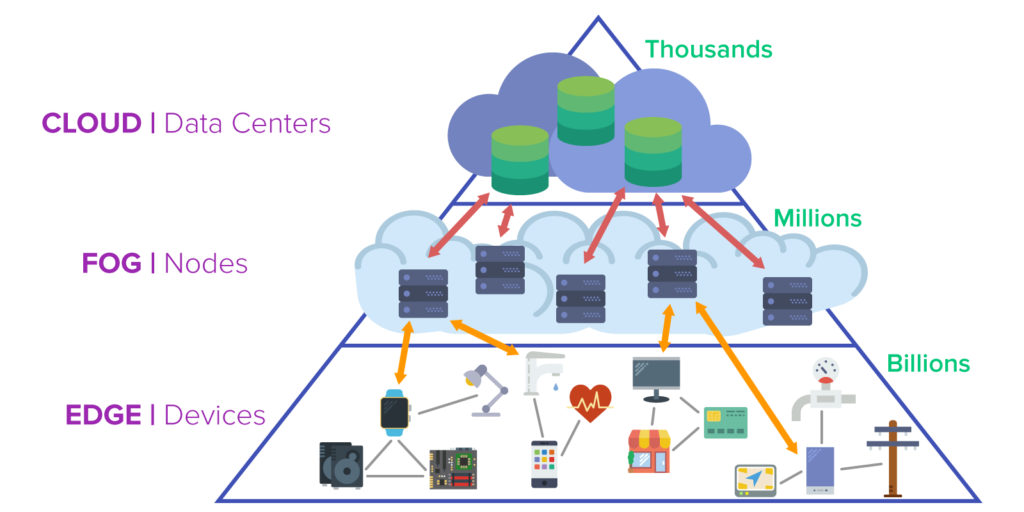
\includegraphics[scale=0.3]{pictures/fogComputingImage.png}
\caption{Arquitetura básica de aplicações que utilizam computação em névoa.}
\label{archFog}
\end{figure}

Seguindo o modelo dessa arquitetura, onde o processamento dos dados deixa de ser feito em apenas um servidor e passa a ser feito nos servidores de borda(fog's, vide figura \ref{archFog}) antes de repassar esses dados para o servidor de armazenamento(cloud, vide figura \ref{archFog}). Portando a arquitetura definida possui os seguintes passos:

\begin{enumerate}
\item Ao iniciar, o servidor de borda deve se registrar no servidor cloud, enviando seus dados.
\item Ao iniciar a conexão, o dispositivo se conecta diretamente ao servidor cloud, que o redireciona para o servidor de borda mais próximo. Já para o médico, o servidor retorna a lista dos pacientes, o médico fica responsável por escolher quem acompanhar e o servidor retorna o endereço ao qual o paciente escolhido está conectado.
\item A partir desse ponto o dispositivo inicia o envio dos dados para o servidor, que o processa e envia periodicamente ao servidor cloud. E o médico ao conectar no servidor recebe diretamente todos os dados do paciente que chegam ao servidor.
\end{enumerate}

Além dessa regra básica a arquitetura define também, que caso o servidor cloud pare de funcionar, os servidores de borda deveram armazenar os dados recebidos, repassando-os quando o servidor de nuvem retornar. Todo o trafego de dados utilizado nessa arquitetura utiliza o protocolo UDP.

Por fim, no protocolo de aplicação, para a tradução dos dados enviados e recebidos o protocolo define alguns códigos no cabeçalho.

\begin{itemize}
\item 00 - Cadastro de dispositivo.
\item 01 - Atualizar status do paciente.
\item 02 - Alterar tempo de atualização.
\item 03 - Conectar conta.
\item 08 - Teste de envio.
\item 09 - Teste de conexão.
\item 00S0 - Cadastro de servidor.
\end{itemize}

\section{Resultados}

Para a primeira aplicação, seguindo a primeira arquitetura, o sistema foi parcialmente entregue, apenas algumas funcionalidades do acompanhamento do médico não foram implementadas.

Com a reestruturação da aplicação seguindo a nova arquitetura, apenas algumas das funcionalidades foram implementadas como os servidores de borda e o servidor de cloud. Onde apenas os dispositivos foram reestruturados, a interface entre médico-servidor e médico-cliente não foi implementada.

\subsection{Conclusões}

O sistema projetado funciona perfeitamente para o acompanhamento do médico, porém para melhorar e fortalecer ainda mais a arquitetura é necessário alterar o protocolo de transporte. Onde a comunicação feita entre dispositivo-cloud, médico-server e médico-cloud deve ser feito em TCP por ser mais confiável. Além de autenticar os médicos no início, para que apenas pessoas cadastradas tenham acesso aos dados dos pacientes nos servidores. E implementar métodos de permanência de dados no cloud.

\bibliographystyle{sbc}
\bibliography{sbc-template}

\end{document}
